\section{Critique of Information Ecosystems}

Several observable and potentially dangerous confusions exist in the two programs outlined above. Fist is the problem in DP where they incorrectly identify Hardin as "the well known ecologist" \citep[][p. 28]{davenport_information_1997}. Hardin was actually a biologist who studied populations of bacteria in petri dishes who is (in)famous for his likening of human populations to bacteria and his over-cited and incorrectly named "Tragedy of the Commons" thesis. According to Elinor Ostrom who shared the 2006 Nobel prize in economics for the her work on property regimes, common pool resources and sustainability, to the correct title to his thesis should be "Tragedy of Open Access" \citep{ostrom_2007}. [need to talk about this]

All share: interconnectedness, contextually dependent, mutual dependencies and causation, interdisciplinary

Not shared: evolutionary

\subsection{Ecologies vs Ecosytems}



\begin{figure}[!ht]
  \centering
    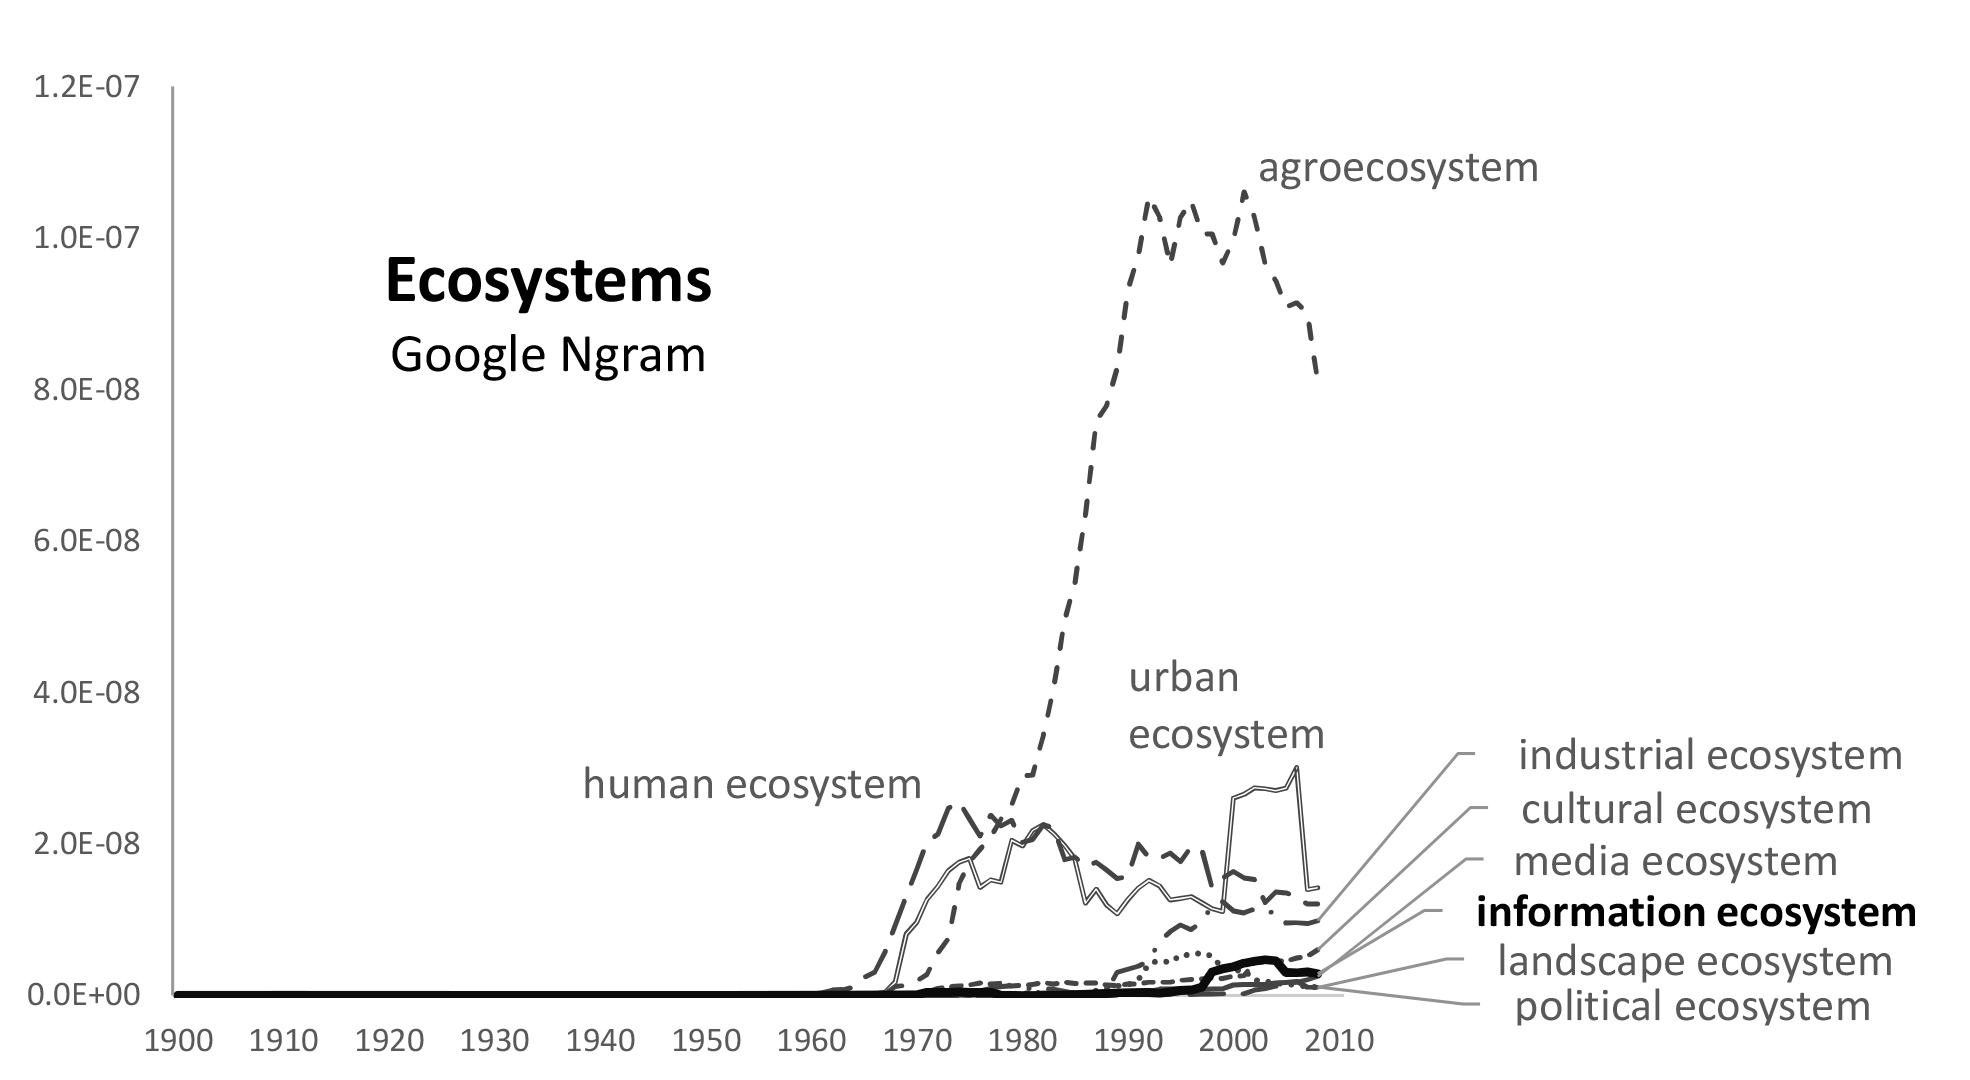
\includegraphics[width=0.9\textwidth]{figures/ecosystemsAll}
  \caption{Emergent use varying ecosystem metaphors as a Google Ngram. Compare to figure 2! The use of ecological metaphors vs ecosystem metaphors is an order of magnitude higher. It is more common to say information ecology (as a study of information systems using ecological concepts) than it is to say information ecosystem (implying a metaphorical relationship).}
\end{figure}

\subsection{Sustainability}

Equivalence between information and energy. From the thermodynamic interpretation of Shannon to later work by Dretske and others moving information into a primary ontological function.

Also equivalence between money (information ecosystems) and energy (real ecosystems)

Sustainability, both environmental and economic - this is actually another major point in the library conversation

\subsection{The attempt to bring humans back into the technology conversation (good!):}

Nardi and O'Day place a great deal of emphasis on the local viewpoint opened up by the concept of information ecology. An explicit motivation for this local focus is to offer an alternative to the system critique of technology, which Nardi and O'Day believe ignores the ways in which people may intervene in technological systems.

NO were writing in the 1990s before the Internet and world wide web became one of the dominant information forces in the world. But they were also writing during the consolidation of the neoliberal Washington consensus in the economic and political realms. In combination I think the growth of neoliberalism and the internet have led to a networked society. Manuel Castells is one of the major sociologists working on this topic. In the networked society local accommodations can quickly be co-opted by larger systemic forces. The argument is that localism is a difficult location from which to build a technical critique of the networked society. Should we be pursuing other avenues? [Other sources than Castells could be used to build this argument, perhaps we need to look to the bibliography for chapter 11 of Kitchin]

\subsection{How is Diversity understood?}

Another important goal for the IE program proposed by NO is to value diversity in information ecologies. DP also discuss the value of diversity for business organizations. But does the idea of diversity really align with the discussion of diversity that occurs in ecology?

- functional diversity (roles of oganisims in an ecosystem)
- species diversity (counts and the shannon/weaver diversity index)
- scale is super important in diversity discussions

\subsection{Greening of the information industry:}

I also believe that a critique could be made of NO and DP that sees the adoption of ecological metaphors as a bit of grandstanding on their part. Identifying with ecology may have a political and rhetorical benefit. Who would want to complain about ecology, especially when the implicit opposite for both NO and DP is a type of technocratic managerialism.

\subsection{Are the emergent properties Natural or set by humans?}

Much of what happens in a data assemblage is conditioned by standards which are mostly developed by institutions and businesses (all human). Is there really room for individuals to intervene at a local level on these standards? And once they are adopted path dependence may set in, making change very difficult.

Another interesting concept to consider in IE is the idea of emergence. Does linking emergence to biological and environmental concepts beneficial [this has been done for a long time, see both Glacken, Worster, Lovelock, etc - hotly debated subject]? These concepts are also present in complexity and chaos studies which tend to have roots in more scientific fields such as physics, and computer science [cybernetics, self governing systems, homeostasis].

\subsection{Are human created phenomena natural}

Within certain critical academic circles naturalizing a phenomena that is a human creation—somehow perceiving the social phenomena as natural—is considered dangerous. A good example might be an explanation of the conquest of Peru as inevitable and ‘natural’ because of superior European weaponry and the disease trajectory from Europe to South America (to simplify a famous argument). Nowhere in this explanation is it mentioned that the conquistadors were social outcasts with a tendency for violence and disrespect of life; perhaps another factor in the conquest. 

"Naturally occuring data" - the social science research council (there is a ref somewhere . . . from Susan Halford at the DCC)

\subsection{Where is Nature in the metaphor?}

Our admittedly incomplete review of the literature suggests that the use of the term information ecosystem either as a metaphor or as a simple vernacular reference actually renders nature more invisible instead of more visible. Is it possible that the use of the term information ecosystem further disconnects us from our natural environment? \citep[cf. ][]{worthy_2013}

\subsection{Human Communities are NOT ecosystems, lack of morality}

One of the uses of the ecosystem metaphor in reearch data management and scholarly communication circles [read libraries] is that scholarly communities are like "ecosystems" through which rivers of data flow \citep{choudhury_2010}. This use of the metaphor invokes a very appealing image of librarians tending the flows of data which pass through scholarly ecosystems nestled within the green hills of the academy. It is perhaps also a dangerously comforting image that borderlines on committing the \textit{Naturalistic Fallacy}; because things are found in nature, they are good. Cognitive scientist Steven Pinker counters this fallacy by noting that possible logical conclusions include statements such as, "if birds and beasts engage in adultry, infanticide, and cannibalism, it must be ok" \citep{pinker_2002}. Another analogous use of the metaphor is that the library itself is an ecosystem in which library specialists, library users, and library professionals interact as different species who have both "competing interests" and relations of "mutual benefit." These relationships lead to a co-evolution of the "species" in a rapidly changing research, publishing and technology environment \citep{walter_2008}. Once again this evokes a sort of touch-feely image where mutualism and cooperation inevitably lead to some sort of outcome that benefits all the "species" involved. Scholarly communities, be it the research community or the library community, are heirarchichal, much like a government agency, with politics and power rippling through their ranks. It is discomforting to think that that, with just a little stretching of these metaphors, the US Department of Defense, or some other government agency, is like an ecosystem through which data flows naturally. The solace to be found with this discomfort comes from the words of Richard Stallman, who launched the free software movement. “It is inadvisable to describe the free software community, or any human community, as an “ecosystem,” because that word implies the absence of ethical judgment.”  Stallman continues:
 
\begin{quote}
The term “ecosystem” implicitly suggests an attitude of nonjudgmental observation: don't ask how [sic] what should happen, just study and understand what does happen. In an ecosystem, some organisms consume other organisms. In ecology, we do not ask whether it is right for an owl to eat a mouse or for a mouse to eat a seed, we only observe that they do so. Species' populations grow or shrink according to the conditions; this is neither right nor wrong, merely an ecological phenomenon, even if it goes so far as the extinction of a species.

By contrast, beings that adopt an ethical stance towards their surroundings can decide to preserve things that, without their intervention, might vanish—such as civil society, democracy, human rights, peace, public health, a stable climate, clean air and water, endangered species, traditional arts … and computer users' freedom. \citep{fsf_2014}
\end{quote}

Perhaps these words also apply to information systems—as these systems are indeed social phenomena—and although the ecosystem metaphor may be convenient and perhaps even practical to describe a scholarly community, we should be careful with expressing an implicit lack of morality in the world of information. 

\subsection{Big Data as Information Pollution}

As our ability increases to capture more quantities of data does the quality decline? As Niel Postman suggests, "We have transformed information [and data] into a form of garbage" \citep[cited in][p. 50]{stepp_1999}. Does this potential decline in quality information somehow hamper effective decision making or are we able to filter and analyze the data in ways that provide novel insights that improve effective decision making?


